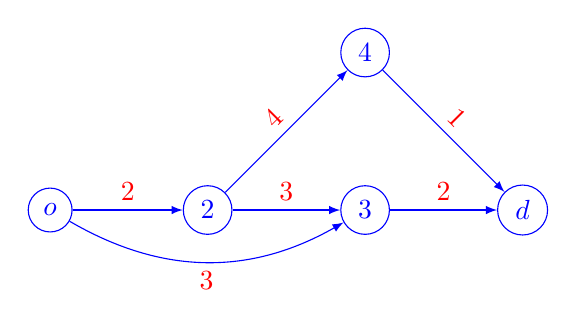
\begin{tikzpicture}[blue, scale=2]
  \node[draw, circle] (V1) at (0,0) {$o$};
  \node[draw, circle] (V2) at (1,0) {$2$};
  \node[draw, circle] (V3) at (2,0) {$3$};
  \node[draw, circle] (V4) at (2,1) {$4$};
  \node[draw, circle] (V5) at (3,0) {$d$};
  
  \draw[-latex] (V1) -- (V2) node[midway,above,red] {$2$};
  \draw[-latex] (V2) -- (V3) node[midway,above,red] {$3$};
  \draw[-latex] (V3) -- (V5) node[midway,above,red] {$2$};
  \draw[-latex] (V2) -- (V4) node[midway,above,sloped,red] {$4$};
  \draw[-latex] (V1) to[bend right] node[midway,below,red] {$3$} (V3) ;
  \draw[-latex] (V4) -- (V5) node[midway,above,sloped,red] {$1$};
\end{tikzpicture}
